\documentclass[12pt]{article}
\usepackage{amsmath,amsfonts,amssymb,graphicx,hyperref}
\usepackage{geometry}
\usepackage{float}
\geometry{a4paper, margin=1in}

\title{\textbf{Improving Blood Alcohol Concentration Models Using the Schnell-Mendoza Equation and Softplus Approximation of the Lambert W Function}}
\author{Nathan Breslow}
\date{\today}

\begin{document}

\maketitle
\thispagestyle{empty}  % Optional: Removes page number from the title page

\begin{abstract}
This paper presents a novel application of the Schnell-Mendoza equation to model alcohol metabolism and improve Blood Alcohol Concentration (BAC) predictions. While the Widmark model assumes a linear elimination rate, alcohol metabolism actually follows Michaelis-Menten kinetics, with enzyme saturation occurring at higher BAC levels (Wilkinson et al., 1976). These kinetics were then analytically solved using the Lambert W function (Schnell and Mendoza, 1997). We synthesize these findings to develop a new BAC prediction model that accurately captures the non-linear nature of alcohol metabolism using the Lambert W function, and introduce a novel approximation method using the softplus activation function (Zheng et al., 2015). We also report a surprising proximity between the ratio of $V_{\text{max}}$ to $K_m$ from Wilkinson et al. and Euler's number, $e$. This paper discusses the derivation of the new model, its computational efficiency, and implications for future research and real-world applications.
\end{abstract}

\section{Introduction}

Accurately modeling Blood Alcohol Concentration (BAC) over time is critical for applications in forensic science, medical toxicology, and public health. The Widmark model has long been the standard approach for estimating BAC based on alcohol consumption, body weight, and time. However, the Widmark model assumes constant alcohol elimination rates - which doesn't make logical sense, as when the concentration of alcohol in the blood is low, the liver is not likely to be metabolizing it at full capacity.

In reality, alcohol metabolism follows Michaelis-Menten kinetics, with enzyme saturation occurring at higher BAC levels. This non-linear behavior is not captured by the Widmark model, leading to inaccuracies in BAC predictions, particularly at low levels. The Schnell-Mendoza equation provides an analytical solution to the Michaelis-Menten system using the Lambert W function, which accurately models the non-linear kinetics of alcohol metabolism.

\section{Background}

\subsection{Widmark Model}
The Widmark formula is widely used to estimate BAC:
\[
\text{BAC} = \frac{A}{rW} - \beta t
\]
where $A$ is the amount of alcohol consumed, $r$ is the Widmark factor, $W$ is body weight, $\beta$ is the elimination rate, and $t$ is the time since consumption. The linear term - $\beta t$ - represents the assumption of constant alcohol elimination. An assumption that has been empirically debunked.

\subsection{Michaelis-Menten Kinetics}
Michaelis-Menten kinetics describe enzyme-catalyzed reactions, such as alcohol metabolism by alcohol dehydrogenase:

\[
    {\displaystyle v={\frac {\mathrm {d} p}{\mathrm {d} t}}={\frac {Va}{K_{\mathrm {m} }+a}}}
\]

where $v$ is the reaction rate, $p$ is the product concentration, $V$ is the maximum reaction rate (also referred to as $V_{\text{max}}$, henceforth these are used interchangeably), $a$ is the substrate concentration, and $K_m$ is the Michaelis constant. 

It can be seen that at low concentrations - as $a$ approaches 0 - the reaction rate is linearly proportional to the substrate concentration:

\[
    {\displaystyle \lim _{a\to 0}{\frac {Va}{K_{\mathrm {m} }+a}}={\frac {V}{K_{\mathrm {m} }}a}}
\]

While as $a$ approaches infinity, the reaction rate approaches $V$:

\[
    {\displaystyle \lim _{a\to \infty }{\frac {Va}{K_{\mathrm {m} }+a}} \approx  \frac{Va}{a} = V}
\]

Thus the model perfectly captures saturable metabolic processes - directly proportional to the substrate concentration at low levels, and constant at high levels.

The values of $V$ and $K_m$ can be determined experimentally, and are specific to the enzyme and substrate in question. For alcohol dehydrogenase, $V_{\text{max}}$ is the maximum rate of alcohol metabolism, and $K_m$ is the concentration of alcohol at which the reaction rate is half of $V$.

Wilkinson et al. (1976) did exactly this by injecting 7 adult men with ethyl alcohol (8\% V/V) for two hours and measuring the rate of alcohol metabolism. The values of $V_{\text{max}}$ and $K_m$ were determined to be 0.0232 mg/(ml x hr) and 0.0082 mg/ml, respectively. The resulting model explained more than 98\% of observed variance in all subjects. Note that the study was only done on men aged 21 to 54, and the numbers could very well be different for women - a promising direction for future research.

\subsection{Schnell-Mendoza Equation}

The Schnell-Mendoza equation provides a closed-form solution to Michaelis-Menten kinetics - specifically for measuring the amount of the substrate concentration $a$ with respect to time: 
\[
a(t) = K_mW_0({\displaystyle{\frac {a_{0}}{K_{\mathrm {m} }}}\exp \!\left({\frac {a_{0}}{K_{\mathrm {m} }}}-{\frac {Vt}{K_{\mathrm {m} }}}\right)})
\]

where $W_0$ is the principal branch of the Lambert W function, and $a_0$ is the initial substrate concentration.

\section{New Model Development}
\subsection{Trivial Model Construction}

It becomes trivial to construct a novel model, as we already have the values of $V_{\text{max}}$ and $K_m$ from Wilkinson et al. (1976) and the Schnell-Mendoza equation. We can simply substitute these values into the equation to get a model that accurately captures the non-linear nature of alcohol metabolism.

Before doing so however, one must note that Wilkinson et. al measured the blood in the capillaries - not the standard venous blood used for BAC. However, a study by Taylor et. al (2020) found that though a statistically significant difference exists between capillary and venous blood on the level of large groups, no such difference exists at the level of individuals. Given that the observed difference was small at the group level and the fact that the coefficients were calculated from only seven people, we can safely ignore this difference.

Thus we get our Schnell-Mendoza model:

\[
b(t) = K_mW_0\left(\frac{b_0}{K_m}\exp\left(\frac{b_0}{K_m} - \frac{Vt}{K_m}\right)\right)
= 
0.0082W_0(\left(\frac{b_0}{0.0082}\exp\left(\frac{b_0}{0.0082} - \frac{0.0232t}{0.0082}\right)\right)
\]

versus the Widmark model of $b(t) = b_0 - 0.015t$.

\begin{figure}[H]
\centering
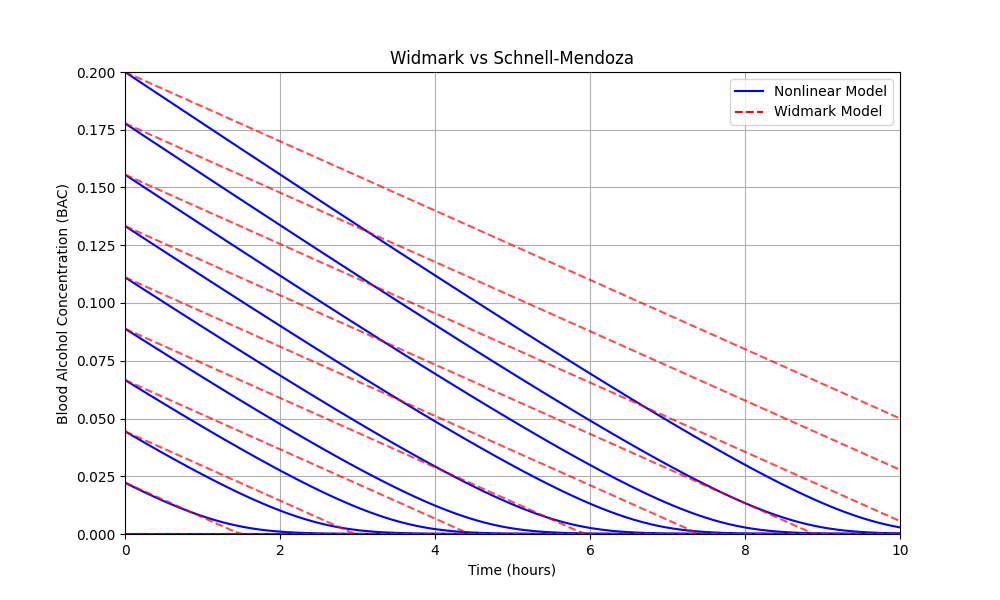
\includegraphics[width=0.8\textwidth]{comparison-schnellmendoza-widmark.png}
\caption{Comparison of Widmark (red), and Schnell-Mendoza (blue) models for BAC over time.}
\label{fig:comparison}
\end{figure}

As seen above, the Schnell-Mendoza model reveals that the Widmark model \textit{overestimates} the speed at which alcohol is metabolized at low BAC levels, and \textit{underestimates} it at high BAC levels - which is the understandable result of attempting to combine the near-zero metabolic rate at low BAC levels with the constant metabolic rate at high BAC levels into a single linear equation. 

The differences are quite distinct - starting at 0.2 BAC, the Widmark model predicts 0.05 BAC remaining in the bloodstream after 10 hours, while the Schnell-Mendoza model predicts near-zero BAC remaining. When starting at 0.02 BAC, the Widmark model predicts complete alcohol absorption after 80 minutes, while Schnell Mendoza predicts that it occurs around roughly 2 hours.

These distinctions may seem minor, but they have real-world implications for both serious applications and recreational drinking.

For instance, this model could be used to more accurately estimate BAC at the time of an incident (when a breathalyzer test is not available) or improve the accuracy of retroactive BAC estimation - important for determining whether someone may have been legally drunk at the time of an incident when the BAC is only calculated hours later. 

In recreational drinking, it provides a more accurate estimate of how long it takes for alcohol to leave the bloodstream - someone going of Widmark would underestimate how fast they'd get drunk if they drank periodically (80 minutes vs 2 hours to clear 0.02 BAC in the example above), and would also overestimate how long it takes for them to sober up (13 hours vs 10 hours to clear 0.2 BAC in the example above).

\subsection{Approximation of Lambert W Function}

Due to the computational complexity of the Lambert W function, we introduce a novel approximation method that words incredibly well over the range of BAC values we are interested in - namely, 0 to 1. The function is as follows:

\[
    b_{approx}(t) = K_m\mathrm{softplus}(-\frac{\frac{\pi + (4 - \pi) \cdot \sqrt{1 - \exp(-e \cdot b_0)}}{4}V}{K_m}t + \frac{b_0}{K_m}) \quad \text{where } \mathrm{softplus}(x) = \log(1 + e^x)
\]

(The derivation of this function will be discussed in the next section.)

The baseline this function is compared to is a simple adaptation of the Widmark model to assume $V$ as the constant rate of metabolism:
\[
    b_{baseline}(t) = b_0 - Vt
\]

The contrast between the three models (the adapted Widmark, the approximation, and the Schnell-Mendoza) is shown below:

\begin{figure}[H]
\centering
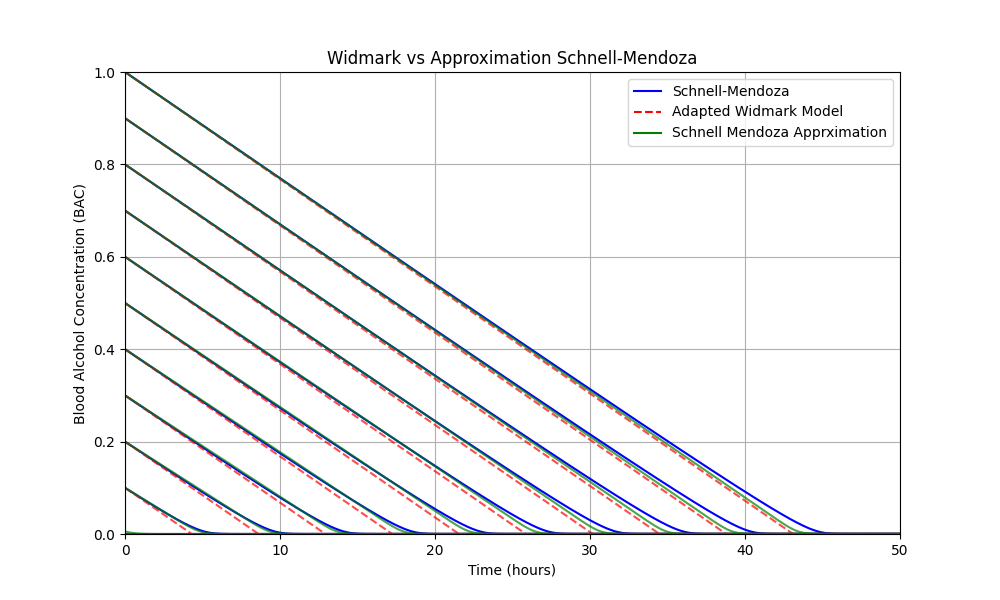
\includegraphics[width=0.8\textwidth]{widmark_vs_approximation.png}
\caption{Comparison of Widmark (red), Approximation (green), and Schnell-Mendoza (blue) models for BAC over time, across all BAC levels.}
\label{fig:comparison}
\end{figure}

Across the full range of BAC levels, 0 to 1, the approximation model is roughly 2.66x more accurate than the adapted Widmark model, as calculated by the mean absolute error.

However, its accuracy improves further if we simply look at BAC levels 0 to 0.2 - a much more realistic range:

\begin{figure}[H]
\centering
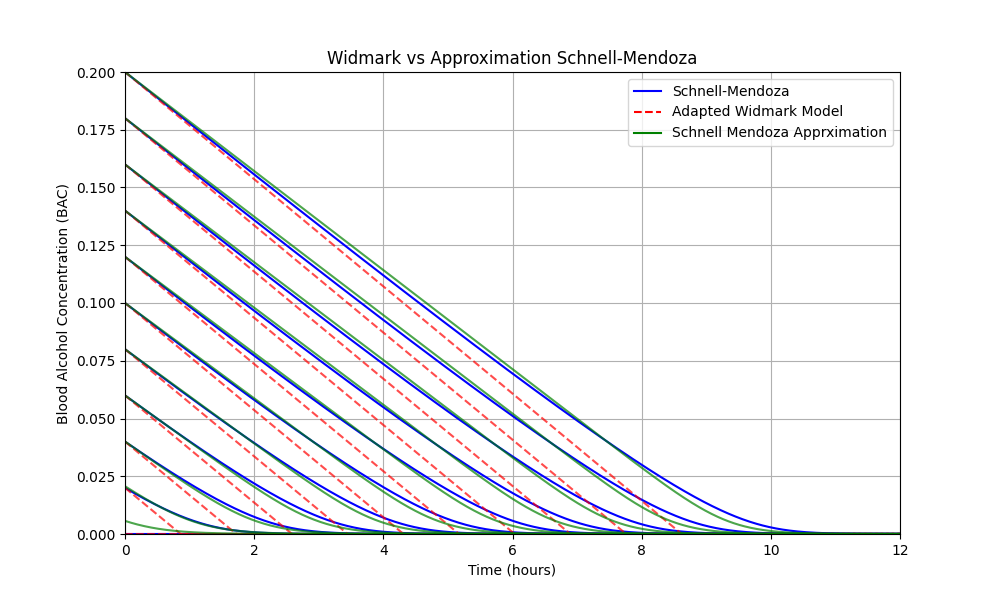
\includegraphics[width=0.8\textwidth]{widmark_vs_approximation_tiny.png}
\caption{Comparison of Widmark (red), Approximation (green), and Schnell-Mendoza (blue) models for BAC over time, across BAC levels 0 to 0.2.}
\label{fig:comparison}
\end{figure}

Here, the approximation model is roughly 4.63x more accurate, as calculated by the mean absolute error.

While the adapted Widmark drastically underestimates the time it takes for alcohol to leave the bloodstream at low BAC levels due to the assumption of a constant metabolic rate at $V_{\text{max}}$, the approximation model accurately captures the non-linear nature of alcohol metabolism, and is computationally efficient, though it still slightly underestimates the time it takes for alcohol to leave the bloodstream at high BAC levels.

The conventional Widmark model fairs far worse - 16.91x less accurate than the approximation model across the range of BAC levels 0 to 0.2. However, one may suggest uniquely fitting a linear model to the Schnell-Mendoza equation, including varying the offset and slope (instead of just the slope).

However - this produces a nonsensical result that at t = 0: the BAC of the approximate linear model wouldn't actually be the initial BAC, but rather a value that results in the best fit to the Schnell-Mendoza model. This is not a desirable property, as the initial BAC is a known value, and the model should reflect that. 

The proposed approximation above does ever-so-slightly vary the initial BAC, but for non-zero BAC values (zero is dramatically overestimated, but that is irrelevant as zero BAC is never practically measured), the variance is, on average, equal to $3 \cdot 10^{-4}$, which is roughly negligible when BAC values are generally measured between $1 \cdot 10^{-2}$ and $2 \cdot 10^{-1}$.

This linear to nonlinear transition is achieved through the clever application of the $softplus$ activation function, which will be discussed in the next section.

\subsection {Derivation of the Approximation}

The Lambert W function is a complex function that is computationally expensive to evaluate - but in this case, it is modeling a fairly simple behavior - namely, linear decay (zeroth order kinetics) becoming exponential decay (first order kinetics) as the BAC level decreases, as is described by Michaelis-Menten kinetics.

The softplus function is defined as:

\[
    \mathrm{softplus}(x) = \ln(1 + e^x)
\]

We can observe its behavior as $x$ approaches infinity - where softplus converges to $x$:

\[
    \lim_{x \to \infty} \ln(1 + e^x) = \lim_{x \to \infty} x
\]

And as $x$ approaches negative infinity softplus converges to $e^x$. We can prove this by first observing that $e^x$ approaches 0 as $x$ approaches negative infinity, and we can then utilize the Taylor series expansion of the natural logarithm plus 1:

\[
    \ln(1 + x) = x - \frac{x^2}{2} + \frac{x^3}{3} - \frac{x^4}{4} + \ldots
\]

Because $e^x$ approaches 0 as $x$ approaches negative infinity, we can simply use the linear approximation of the natural logarithm:

\[
    \ln(1 + e^x) \approx e^x \quad \text{as } e^x \to 0, x \to -\infty
\]

Thus, we see that the softplus function is a smooth transition from exponential to linear behavior - approaching $e^x$ as $x$ approaches negative infinity, and $x$ as $x$ approaches positive infinity. This is exactly what we need to approximate the Lambert W function here - a smooth transition from linear to exponential behavior.

Now that we have our function, we must determine how to manipulate it in order to approximate the Schnell-Mendoza equation.

Let us first look at a simplified version of the approximation:

\[
    b_{approx}(t) = K_m\mathrm{softplus}(-\frac{V}{K_m}t + \frac{b_0}{K_m})
\]

This approximation specifically works well for the empirically determined values of $V_{\text{max}}$ and $K_m$ from Wilkinson et al. (1976) - 0.0232 and 0.0082 respectively. The reason is as follows:

Provided that the argument to softplus is sufficiently large, $\mathrm{softplus}(x)$, as shown above, can be approximated as $x$. So for $t = 0$:

\[
    K_m\mathrm{softplus}(-\frac{V}{K_m}{0} + \frac{b_0}{K_m}) \approx K_m( \frac{b_0}{K_m}) = b_0
\]

Thus our function starts at the initial BAC level, as desired.

Furthermore, notice that when the argument to softplus is large enough - a linear model emerges:

\[
    K_m\mathrm{softplus}(-\frac{V}{K_m}t + \frac{b_0}{K_m}) \approx K_m(-\frac{V}{K_m}t + \frac{b_0}{K_m}) = b_0 - Vt
\]

Which is simply the Widmark model.

on the other hand, when the argument to softplus is small enough - an exponential model emerges:

\[
    K_m\mathrm{softplus}(-\frac{V}{K_m}t + \frac{b_0}{K_m}) \approx K_m\exp(-\frac{V}{K_m}t + \frac{b_0}{K_m})
\]

The transition to the exponential model occurs as the remaining amount of alcohol predicted by the linear model approaches zero - which is exactly what we want.

$K_m$ here serves as a scaling factor - arbitrarily inflating the initial value of $b_0$ into a range that causes $\mathrm{softplus}$ to produce an initially linear output. This mirrors the role of $K_m$ in Michaelis-Menten kinetics - where it mediates the length of the transition between exponential and linear behavior - with large $K_m$ values causing the transition to occur over a longer period of time. In this approximation, larger $K_m$ values also cause this, as they reduce the amount the input to $\mathrm{softplus}$ is scaled by and thus increase the period of time over which the transition from exponential to linear behavior occurs.

Note that $\frac{b_0}{K_m}$ must be significantly larger than $0$ for the approximation to work - as the softplus function is only linear for large values of $x$. This explains the overestimation at zero BAC - as the approximation is not valid for values of $b_0$ extremely close to zero. It also breaks down for high values of $K_m$ - as the scaling becomes far too slow and the approximation becomes inaccurate. However, for the empirically found constants and BAC levels of interest, the approximation is incredibly accurate.

There exists one additional component of the approximation that is not immediately obvious - the $\frac{\pi + (4 - \pi) \cdot \sqrt{1 - \exp(-e \cdot b_0)}}{4}$ term. The fact is this is an arbitrarily selected scaling term to improve the accuracy of the approximation. Why so complex? Well, it became evident that the coefficient of $t$ should be dependent on $b_0$ to reduce error upon initial testing, so we fitted polynomials from 0 to 10 degrees in order to better understand the relationship between $b_0$ and the optimal coefficient of $t$ - effectively trying to find function $f$ such that:

$$
    b_{approx}(t) = K_m\mathrm{softplus}(-f(b_0)\frac{V}{K_m}t + \frac{b_0}{K_m})
$$

The polynomials converged to a function that started at roughly $\frac{\pi}{4}$ (around 0.78-0.82, $\frac{\pi}{4}$ was chosen because its a pretty number) when $b_0$ , and converged to 1 as $b_0$ approached 1. This led to the development of an exponential interpolation model between $\frac{\pi}{4}$ and 1:

$$
    \frac{\pi + (4 - \pi) \cdot \sqrt{1 - \exp(-k \cdot b_0)}}{4}
$$

where $k$ is a constant that determines the rate of convergence to 1. $k$ was empirically determined to be roughly 2.73, and substituting $k$ for $e$ did not significantly change the accuracy of the approximation, giving us:

$$
    \frac{\pi + (4 - \pi) \cdot \sqrt{1 - \exp(-e \cdot b_0)}}{4}
$$

Because empirically determined constants can often be messy, the goal here was to find some version of $f(b_0)$ such that the majority of numbers involved in the function were simple integers or common mathematical constants, instead of extremely precise decimals. While accuracy may be ever-so-slightly reduced (by a value so miniscule as to be below statistical significance), the function becomes far more readable and understandable.

To provide empirical evidence, the average error on $t$ values ranging from 0-20 and $b_0$ values ranging from 0-1 was calculated for both the elegant approximation and an optimally fitted 8th-degree polynomial approximation. The elegant approximation had an average error of $8.14 \cdot 10^{-4}$, while the polynomial approximation had an average error of $7.29 \cdot 10^{-4}$. This amounts to a difference of $0.85 \cdot 10^{-5}$, which is so small that there's clearly little benefit to including eight highly specific constants in the model.



Thus the final form of the approximation was determined to be:

\[
    b_{approx}(t) = K_m\mathrm{softplus}(-\frac{\frac{\pi + (4 - \pi) \cdot \sqrt{1 - \exp(-e \cdot b_0)}}{4}V}{K_m}t + \frac{b_0}{K_m})
\]

Note that there could be better approximations out there for the Schnell-Mendoza equation w/out using the Lambert W function, but this one is particularly elegant and simple, and it works incredibly well for the empirically determined values of $V_{\text{max}}$ and $K_m$ from Wilkinson et al. (1976).

To ensure that this wasn't the only piece of low-hanging fruit, an exhaustive search was performed using genetic algorithms to perform discrete program synthesis - the python library \texttt{deap} was employed, and the algorithm was given access to several key primitives - all elementary operations, $\log$ and $\exp$, and $V$ and $K_m$. The solution space was restricted to monotonically decreasing functions that started at $b_0$ and converged to 0 after initial results were poor. Multiple hyperparameters were tested - the population size was varied from 100 to 1000, the number of generations was varied from 50 to 500, and a variety of mutation rates were tested. 

Despite all these efforts, no discovered functions came anywhere close to the accuracy of the softplus approximation, regardless of the starting hyperparameters. Thus, we confidently conclude that the softplus approximation cannot be trivially surpassed by simple program search and thus represents a meaningful contribution to the field.


\subsection{Implications and Applications}
Our model has significant implications for fields that rely on BAC estimation. As mentioned earlier, legal proceedings that involve retroactive BAC estimation or BAC estimation w/out breathalyzer results may benefit from the greater accuracy of this model - especially when initial BAC levels are low or the BAC levels involved are at the tail end of the metabolic process.

In medical contexts, accurate BAC prediction can aid in determining appropriate treatment times or medication interactions. Furthermore, the existence of the softplus approximation is allows  edge devices - such as a smart watch or phone - to accurately estimate BAC levels in real-time. The softplus approximation additionally utilizes operations like $\exp$ and $\log(1 + x)$ that are already optimized in modern hardware, making it computationally efficient and suitable for real-time applications.

\section{Future Work & Limitations}
The surprising proximity of the $V_{\text{max}}/K_m$ ratio to $e$ warrants further investigation - the ratio of the constants found by Wilkinson et al. (1976) is roughly 2.83, while Euler's number is 2.71828. Furthermore, the fact that the optimal constant for the exponential interpolation model was roughly 2.73 is intriguing, and also hints at a potential relationship between the constants of Michaelis-Menten kinetics and Euler's number.

Future research should explore the biological implications of this relationship and determine if it holds across different metabolic processes - do the $V_{\text{max}}/K_m$ ratios of other enzymes in the body also approximate Euler's number? If so, what does this mean for the underlying biology of metabolic systems?

Additionally, the softplus approximation could be further optimized for different ranges of substrate values or different metabolic systems - as right now it is specifically tailored to the empirically determined values of $V_{\text{max}}$ and $K_m$ from Wilkinson et al. (1976). A more general approximation that works across a wider range of values would be beneficial for applications in pharmacokinetics and computational modeling.

Furthermore, the Wilkinson model - and the Schnell-Mendoza equation that arises from it - has not yet been validated on a larger sample size independently. This is a critical step in ensuring the accuracy of the model and its applicability to a wider range of individuals - until then, the improvements proposed in this paper to the Widmark model are purely theoretical, as the Schnell-Mendoza equation is taken as ground truth.

Finally, the study that Wilkinson et al. (1976) conducted was only done on healthy adult men, and the values of $V_{\text{max}}$ and $K_m$ could be different for women, elderly individuals, children, or individuals with certain medical conditions. Future research should investigate the values of these constants across different populations and determine how they affect the accuracy of BAC prediction models.

\section{Conclusion}
This paper presents a novel application of the Schnell-Mendoza equation to alcohol metabolism and introduces a computationally efficient approximation of the Lambert W function using the softplus activation function within the domain of BAC prediction. The model improves significantly over the Widmark model, particularly at low BAC levels, and raises intriguing questions about the role of Euler's number in metabolic systems. This work lays the foundation for further research in mathematical biology, pharmacokinetics, and computational modeling.

\pagebreak

\bibliographystyle{plain}
\bibliography{references}

\begin{thebibliography}{9}

\bibitem{Widmark1932} 
Widmark, E. M. P. (1932). 
\textit{Die theoretischen Grundlagen und die praktische Verwendbarkeit der gerichtlich-medizinischen Alkoholbestimmung}. 
Urban \& Schwarzenberg, Berlin.

\bibitem{Wilkinson1976}
Wilkinson, P. K., Sedman, A. J., Sakmar, E., Earhart, R. H., Weidler, D. J., \& Wagner, J. G. (1976). Blood ethanol concentrations during and following constant‐rate intravenous infusion of alcohol. \textit{Clinical Pharmacology \& Therapeutics}, 19(2), 213–223. https://doi.org/10.1002/cpt1976192213

\bibitem{Schnell1997} 
Schnell, S., \& Mendoza, C. (1997). Closed form solution for time-dependent enzyme kinetics. \textit{Journal of Theoretical Biology}, 187(2), 207–212. https://doi.org/10.1006/jtbi.1997.0425 

\bibitem{Zheng2015} 
Zheng, H., Yang, Z., Liu, W., Liang, J., \& Li, Y. (2015). Improving deep neural networks using Softplus units. \textit{2015 International Joint Conference on Neural Networks (IJCNN)}, 15, 1–4. https://doi.org/10.1109/ijcnn.2015.7280459 

\bibitem{Taylor2020} 
Taylor, L., Remeškevičius, V., Saskoy, L., Brodie, T., Mahmud, J., Moir, H., Brouner, J., Howe, C., Thatti, B., Connell, S. O., Trotter, G., \& Rooney, B. (2020). Determination of ethanol in micro-volumes of blood by headspace gas chromatography: Statistical comparison between capillary and venous sampling sites. \textit{Medicine, Science and the Law}, 61(2), 86–96. https://doi.org/10.1177/0025802420928632 

\end{thebibliography}



\end{document}
